\section*{Termocupla y sus ejemplos de aplicación}

Una termocupla es un sensor de temperatura robusto y ampliamente utilizado que se basa en el efecto Seebeck: cuando dos metales distintos se unen en un extremo (llamado "unión caliente" o de medida) y ese punto se somete a un gradiente de temperatura respecto al otro extremo ("unión fría" o de referencia), se genera un pequeño voltaje eléctrico directamente proporcional a esa diferencia de temperatura. Este milivoltaje, característico de la combinación de metales utilizada, es medido por un instrumento indicador o controlador, que lo traduce a un valor de temperatura. Su importancia radica en su simplicidad, amplio rango de medición, capacidad para responder rápidamente a cambios de temperatura y su notable robustez, ya que no requieren fuente de alimentación externa para generar la señal.

\subsection*{Ejemplos de aplicación}

Dentro de las aplicaciones para las termocuplas se puede estimar 3 ejemplos destacados en el que la generación de energía eléctrica a partir de la diferencia de temperatura en un los conductores es relevante para el funcionamiento de los circuitos deseados.

 \begin{itemize}
 	\item Control de hornos y altas temperaturas en la industria: En la siderurgia, fabricación de cerámica o tratamientos térmicos, las termocuplas tipo B, S o K son esenciales por su capacidad de medir desde cientos hasta más de 1700°C. Se instalan directamente en las cámaras de combustión o paredes del horno para garantizar el ciclo térmico exacto del material.
 	\item Monitoreo en sistemas de turbinas y motores: En la industria de generación de energía y aeronáutica, se utilizan termocuplas, a menudo tipo J o K, para medir la temperatura de gases de escape en turbinas o la temperatura de cilindros en motores. Estos datos son críticos para el control automático del rendimiento, la eficiencia del combustible y la prevención de sobrecalentamientos que podrían causar fallas catastróficas.
 	\item Instrumentación en laboratorios y procesos farmacéuticos: Por su rapidez de respuesta y versatilidad, las termocuplas tipo T (para bajas temperaturas) o K son comunes en baños de temperatura, cámaras de estabilidad, esterilizadores y equipos de secado. Permiten validar y controlar con precisión las condiciones ambientales requeridas en procesos sensibles, donde la trazabilidad y la exactitud son fundamentales para la calidad del producto.
 \end{itemize}
 
 \section*{Partes de una termocupla industrial}
 
 Una termocupla de laboratorio suele ser un sensor básico, con los dos hilos metálicos desnudos o con un aislamiento delgado (como fibra de vidrio o PTFE), expuesta y frágil, diseñada para ambientes controlados. En contraste, una termocupla industrial se distingue por su robustez y protección para entornos hostiles. Sus características clave incluyen una vaina metálica (generalmente de acero inoxidable, inconel u otras aleaciones) que encapsula y protege herméticamente la unión de medida y los hilos, aislamientos minerales compactados (óxido de magnesio o alúmina) para alta estabilidad y resistencia a vibraciones, y una cabeza de conexión estanca que protege los terminales de humedad y polvo. Además, suele tener una conexión de proceso (rosca, brida o fijación) para una instalación segura y repetible en tanques, tuberías o equipos, soportando presiones, vibraciones, atmósferas corrosivas y temperaturas extremas de forma continua y fiable.
 
 \begin{figure}[h]
 	\centering
 	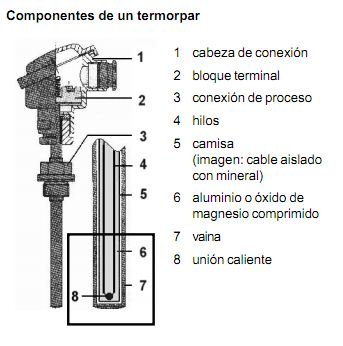
\includegraphics[width=0.5\linewidth]{media/termopar-industrial}
 	\caption{Termopar industrial}
 	\label{fig:termopar-industrial}
 \end{figure}
 
 En la figura \ref{fig:termopar-industrial} se muestra un termopar/termocupla industrial con sus partes correspondientes mediante un diagrama esquemático que desglosa los componentes clave de una termocupla industrial con aislamiento mineral y vaina metálica. En la parte superior se identifica la cabeza de conexión (1), que alberga el bloque terminal (2) donde se realizan las conexiones eléctricas seguras. Desde ahí, el conjunto se extiende mediante una conexión de proceso (3), que permite el montaje en equipos, mientras que la parte central o núcleo del sensor muestra los dos hilos (4) de metales distintos (que forman el par termoeléctrico), aislados individualmente por un material compactado, identificado como aluminio o óxido de magnesio comprimido (6), dentro de una vaina metálica protectora (7). Todo este conjunto constituye el cable con camisa (5). En el extremo inferior de la vaina, los hilos se fusionan para formar la unión caliente (8), el punto donde realmente se mide la temperatura. Este diseño garantiza durabilidad, respuesta rápida y protección integral del elemento sensor.